%=========================================================
\chapter{Diseño Arquitectónico}
\label{cap:reqUsr}

	En este capítulo se modela el alcance del sistema. Se presentan inicialmente los Actores involucrados y sus requerimientos, especificando cuales se alcanzaron en la primera iteración y cuales serán trabajados en la segunda iteración. Después se presentan los requerimientos funcionales de esta iteración y al final se presenta el modelo Físico y Lógico del sistema.


%---------------------------------------------------------
\section{Entorno de Producción}
\cdtInstrucciones{
	Identifique los actores que estarán involucrados en los procesos relacionados con el sistema para esta iteración de desarrollo. Ponga énfasis en los procesos involucrados.
}

\subsection{Organigrama de la Empresa}
\begin{figure}[htbp]
	\begin{center}
		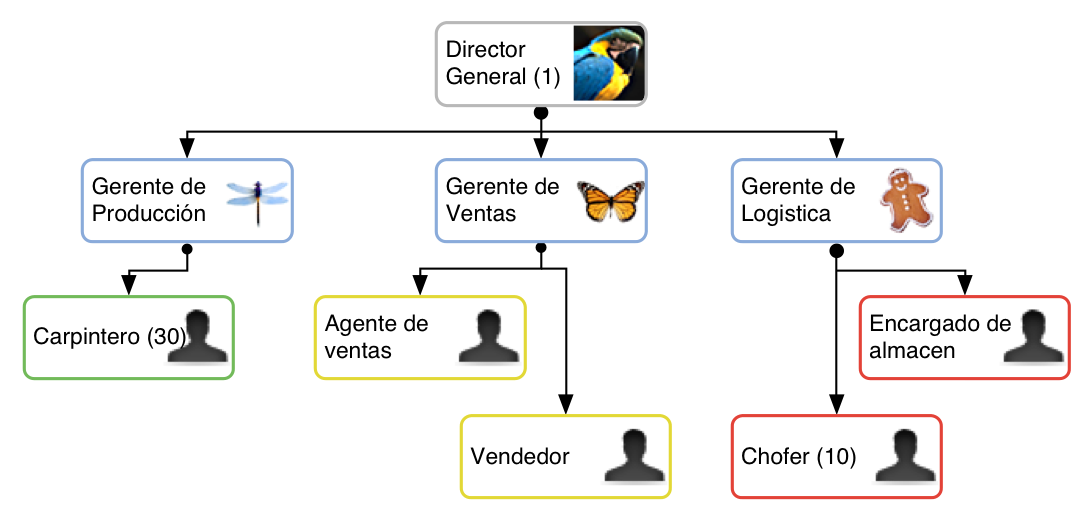
\includegraphics[width=.8\textwidth]{images/organigramaEm}
		\caption{Organigrama de la Mueblería Qetzal S. A. de C. V.}
		\label{fig:organigrama}
	\end{center}
\end{figure}


%---------------------------------------------------------
\begin{Usuario}{\subsection{Gerente de Ventas}}{
	Es el encargado de todas las operaciones de ventas al mayoreo y al menudeo. coordina y supervisa el trabajo de los Agentes de Ventas y Encargados de Tienda.
	Reporta directamente al Gerente de Operaciones
}
    \item[Responsabilidades:] \cdtEmpty
    \begin{itemize}
		\item Supervisar la operación de ventas.
		\item Plantear y supervisar el logro de las metas de ventas de la empresa y su crecimiento económico.
		\item ...
    \end{itemize}

	\item[Perfil:] \cdtEmpty
    \begin{itemize}
		\item Amplia experiencia en el ramo.
		\item Licenciatura como mínimo.
		\item ...
    \end{itemize}
	\item[Procesos en los que participa:] \cdtEmpty
    \begin{itemize}
		\item PC-V01 Aprobar las ordenes de compra al mayoreo.
		\item PC-V02 Supervisar las ventas al menudeo.
		\item PC-V03 Elaborar informe de ventas mensual.
		\item ...
    \end{itemize}
\end{Usuario}

%---------------------------------------------------------
\begin{Usuario}{\subsection{Agente de Ventas}}{
	...
}
    \item[Responsabilidades:] \cdtEmpty
    \begin{itemize}
		\item ...
    \end{itemize}

	\item[Perfil:] \cdtEmpty
    \begin{itemize}
		\item ...
    \end{itemize}
	\item[Procesos en los que participa:] \cdtEmpty
    \begin{itemize}
		\item PC-V08 Venta al Mayoreo.
		\item ...
    \end{itemize}
\end{Usuario}


%---------------------------------------------------------
\section{Entorno de Desarrollo}

\cdtInstrucciones{
	Identifique y describa los requerimientos funcionales del sistema señalando: id, nombre, descripción y prioridad.
}

\begin{table}[htbp!]
	\begin{requerimientosU}
		\FRitem{RU1}{Control de vehículos}{El usuario requiere llevar un registro actualizado de los vehículos, sus características y su estado.}{1}{\DONE}
		\FRitem{RU2}{Registro de ventas}{El usuario requiere llevar un registro actualizado de todas las ventas realizadas por mes y su status: pedido, entregado, pagado, etc..}{2}{\TODO}
		\FRitem{RU3}{Registro de clientes}{El usuario requiere llevar un registro actualizado de todos los clientes para su seguimiento, atención y tareas de promoción y mercadotecnia.}{1}{\DONE}
		\FRitem{RU4}{Planeación de entregas}{El usuario requiere una herramienta que le facilite la planeación de vehículos para que esta sea la más adecuada.}{-}{\PLAN}
		\FRitem{...}{...}{...}{...}{...}
	\end{requerimientosU}
    \caption{Requerimientos funcionales del sistema.}
    {\footnotesize\em Para leer correctamente esta tabla vea la leyenda en la Tabla~\ref{tbl:leyendaRF} en la página~\pageref{tbl:leyendaRF}.}
    \label{tbl:reqFunc}
\end{table}



%---------------------------------------------------------
\section{Lanzamientos de Diseño}	

\cdtInstrucciones{
	Coloque un diagrama y su descripción para aclarar el tipo de solución propuesta. \\
	
 En esta sección se debe aclarar:
	
\begin{description}
	\item[Tipo de sistema:] Web, aplicación móvil, de escritorio, híbrida, etc.
	\item[Software requerido:] Programas que se deberán instalar, desde el sistema operativo, compiladores, interpretes, servidores, etc.
	\item[Hardware requerido:] CPU, núcleos, velocidad, memoria, disco duro, etc.
	\item[servicios:] De conexión, seguridad, firewall, respaldo de energía, redundancia, uso de raids, etc.
\end{description}
}

\begin{figure}[htbp!]
	\begin{center}
		\fbox{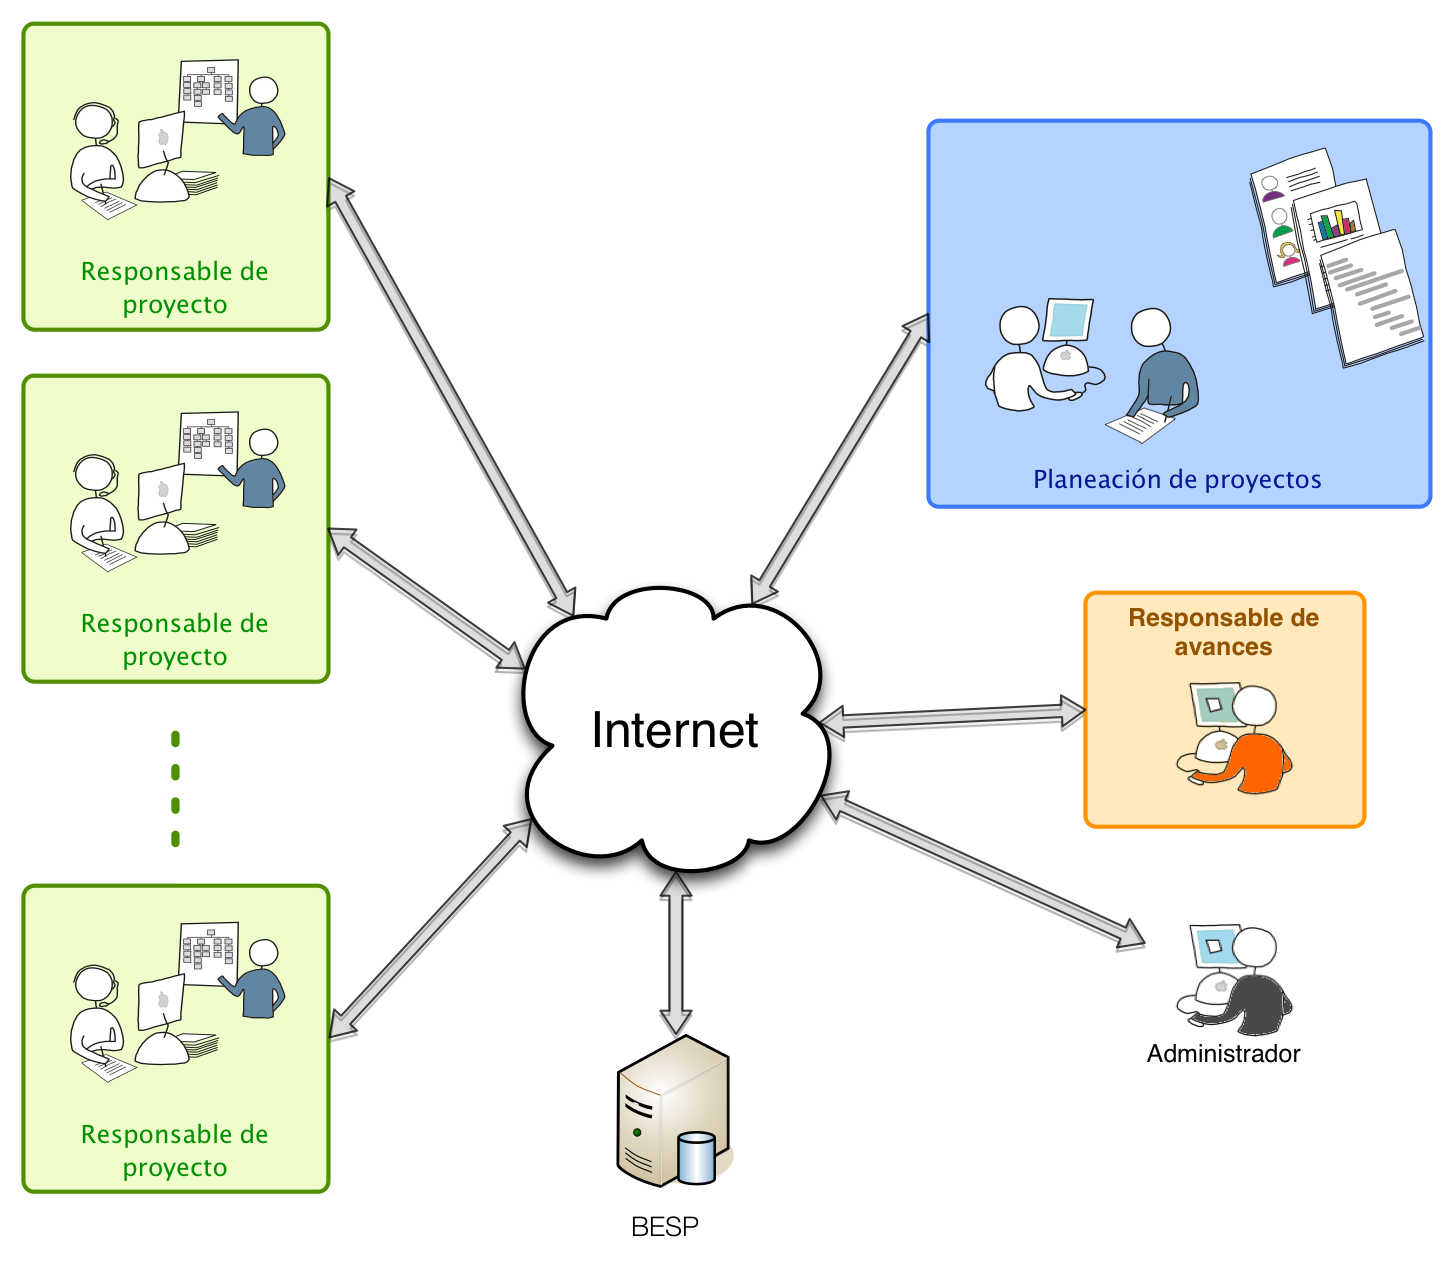
\includegraphics[width=.6\textwidth]{images/arquitectura}}
		\caption{Arquitectura del sistema.}
		\label{fig:arquitectura}
	\end{center}
\end{figure}

En la figura~\ref{fig:arquitectura} se describe la estructura del sistema, en ella se detalla ...


